% Options for packages loaded elsewhere
\PassOptionsToPackage{unicode}{hyperref}
\PassOptionsToPackage{hyphens}{url}
%
\documentclass[
]{article}
\usepackage{lmodern}
\usepackage{amssymb,amsmath}
\usepackage{ifxetex,ifluatex}
\ifnum 0\ifxetex 1\fi\ifluatex 1\fi=0 % if pdftex
  \usepackage[T1]{fontenc}
  \usepackage[utf8]{inputenc}
  \usepackage{textcomp} % provide euro and other symbols
\else % if luatex or xetex
  \usepackage{unicode-math}
  \defaultfontfeatures{Scale=MatchLowercase}
  \defaultfontfeatures[\rmfamily]{Ligatures=TeX,Scale=1}
\fi
% Use upquote if available, for straight quotes in verbatim environments
\IfFileExists{upquote.sty}{\usepackage{upquote}}{}
\IfFileExists{microtype.sty}{% use microtype if available
  \usepackage[]{microtype}
  \UseMicrotypeSet[protrusion]{basicmath} % disable protrusion for tt fonts
}{}
\makeatletter
\@ifundefined{KOMAClassName}{% if non-KOMA class
  \IfFileExists{parskip.sty}{%
    \usepackage{parskip}
  }{% else
    \setlength{\parindent}{0pt}
    \setlength{\parskip}{6pt plus 2pt minus 1pt}}
}{% if KOMA class
  \KOMAoptions{parskip=half}}
\makeatother
\usepackage{xcolor}
\IfFileExists{xurl.sty}{\usepackage{xurl}}{} % add URL line breaks if available
\IfFileExists{bookmark.sty}{\usepackage{bookmark}}{\usepackage{hyperref}}
\hypersetup{
  pdftitle={Estimating the time-varying reproduction number of SARS-CoV-2 using national and subnational case counts},
  hidelinks,
  pdfcreator={LaTeX via pandoc}}
\urlstyle{same} % disable monospaced font for URLs
\usepackage[margin=1in]{geometry}
\usepackage{graphicx,grffile}
\makeatletter
\def\maxwidth{\ifdim\Gin@nat@width>\linewidth\linewidth\else\Gin@nat@width\fi}
\def\maxheight{\ifdim\Gin@nat@height>\textheight\textheight\else\Gin@nat@height\fi}
\makeatother
% Scale images if necessary, so that they will not overflow the page
% margins by default, and it is still possible to overwrite the defaults
% using explicit options in \includegraphics[width, height, ...]{}
\setkeys{Gin}{width=\maxwidth,height=\maxheight,keepaspectratio}
% Set default figure placement to htbp
\makeatletter
\def\fps@figure{htbp}
\makeatother
\setlength{\emergencystretch}{3em} % prevent overfull lines
\providecommand{\tightlist}{%
  \setlength{\itemsep}{0pt}\setlength{\parskip}{0pt}}
\setcounter{secnumdepth}{-\maxdimen} % remove section numbering

\title{Estimating the time-varying reproduction number of SARS-CoV-2 using
national and subnational case counts}
\author{}
\date{\vspace{-2.5em}}

\begin{document}
\maketitle

\textbf{Authors:} Sam Abbott *, Joel Hellewell *, Robin N Thompson,
Katharine Sherratt, Hamish P Gibbs, Nikos I Bosse, James D Munday,
Sophie Meakin, Emma L Doughty, June Young Chun, Yung-Wai Desmond Chan,
Flavio Finger, Paul Campbell, Akira Endo, Carl A B Pearson, Amy Gimma,
Tim Russell, CMMID COVID modelling group, Stefan Flasche, Adam J
Kucharski, Rosalind M Eggo, Sebastian Funk

* contributed equally

\hypertarget{abstract}{%
\section{Abstract}\label{abstract}}

\textbf{Background:} Assessing temporal variations in transmission in
different countries is essential for monitoring the epidemic, evaluating
the effectiveness of public health interventions and estimating the
impact of changes in policy.

\textbf{Methods:} We use case notification data to generate daily
estimates of the time-dependent reproduction number subnationally and
nationally. Our modelling framework, based on open source tooling,
accounts for uncertain reporting delays, so that the reproduction number
is estimated based on underlying latent infections and not reported
cases.

\textbf{Results:} We provide three example uses of our framework. First,
we demonstrate how the toolset displays temporal changes in the
reproduction number. Second, we show how the framework can be used to
reconstruct case counts by date of infection from case counts by date of
notification, as well as to estimate the reproduction number. Third, we
show how maps can be generated to clearly show if case numbers are
likely to decrease or increase in different regions. Results are shown
subnatioanlly and nationally on our website
(\url{https://epiforecasts.io/covid/}) and are updated regularly. Our
tooling is provided as an open-source R package to allow replication by
others.

\textbf{Conclusions:} This decision-support tool can be used to assess
changes in virus transmission both subnationally and nationally. This
allows public health officials and policymakers to track the progress of
the outbreak in near realtime using a epidemioligcally valid measure. As
well as providing regular updates on our website, we also provide an
open source toolset so that our approach can be used directly by
researchers and policymakers on confidential datasets. We hope that our
tool will be used to support decisions in countries worldwide throughout
the ongoing COVID-19 pandemic.

\textbf{Keywords}: Covid-19, SARS-CoV-2, surveillance, forecasting,
time-varying reproduction number

\hypertarget{introduction}{%
\section{Introduction}\label{introduction}}

The coronavirus disease 2019 (COVID-19) pandemic that emerged in
December 2019 has since spread to over 100 countries in every continent
except Antarctica. While some information on the progress of an outbreak
in a given country can be gained from the reported numbers of confirmed
cases and deaths, these numbers can obscure changes in the underlying
dynamics of the outbreak due to delays between infection and the
eventual reporting of a case or death. Accounting for the uncertain
delays from infection to symptom onset, and the uncertain delays from
symptom onset to hospital admission, diagnostic testing or potential
death, followed by further delays until data are recorded in official
statistics, requires the use of specific statistical methods for
handling right-truncated data {[}1--3{]},uncertainty, and the creation
of a ``nowcast'' {[}4,5{]} (an estimate of the current number of newly
infected or symptomatic cases).

A method for tracking the progress of an outbreak is to measure changes
in the time-varying reproduction number (effective reproduction number),
which represents the average number of secondary infections generated by
each new infectious case {[}6--8{]}. This approach can be advantageous
compared to monitoring numbers of newly reported or symptomatic cases
since, in principle, reproduction number estimates reflect variations in
transmission intensity. Due to the delays in disease progression,
recorded numbers of newly notified or symptomatic cases will increase or
decrease for a period after transmissibility has reduced or increased,
respectively. Monitoring changes in the time-varying reproduction can
account for this delay and reveals variations in transmissibility that
are not clear when using only reported cases.

This paper outlines the website we have developed
(\url{https://epiforecasts.io/covid/}) that presents estimates and
forecasts of reported cases by date of infection and the respective
time-varying reproduction numbers both nationally and subnationally.
This website relies on methods implemented in the \texttt{EpiNow2} R
package and data aggregated in the \texttt{covidregionaldata} R package,
both developed by the authors {[}9,10{]}. Our approach is based on
reported cases counts (though we provide estimates based on both
reported cases and deaths) and data on the delay between infection and
symptom onset and symptom onset and report. We use a bayesian latent
variable approach to estimate infections from prior infections, an
estimate of the generation time and the time-varying reproduction number
{[}6,11{]}. Temporal variation in the reproduction number estimates
controlled using a Gaussian process. Reported cases are then
extrapolated by convolving by the uncertain incubation period and delay
between symptom onset and case report (or death when estimating using
deaths). Uncertainty in reporting is captured using a negative binomial
reporting model that includes day of the week effects. By extending the
covariance matrix of the gaussian process we derive a forecast of
potential reproduction number trajectories and infections. We combine
this approach with ensembles of timeseries models {[}12{]}. We then use
open-source Rmarkdown templates and the distill framework to generate a
webpage summarising these estimates {[}{\textbf{???}},{\textbf{??}}{]}
and present them as downloadable csvs under an open-source license for
use elsewhere. Our estimates overcome some of the limitations of more
naive implementations that derive estimates for the reproduction number
directly from numbers of reported cases without adjusting (or with only
partial adjustment) for the delay from infection to symptom onset or
from onset to notification. Our approach also incorporates multiple
sources of uncertainty that if excluded can bias estimates. The code
that creates and updates the website is open source, allowing
policymakers and researchers to run analyses in private repositories
using confidential data. The methods outlined in this paper and
corresponding code base are under development, and new versions of this
live article will be released alongside changes to the methods to create
a record of the methodology used throughout the pandemic.

\hypertarget{methods}{%
\section{Methods}\label{methods}}

\hypertarget{data}{%
\subsection{Data}\label{data}}

We use daily counts of confirmed cases and deaths reported by the
European Centre for Disease Control from the last 12 weeks for all
analyses conducted at the national level {[}10,13{]}. To estimate the
delay from symptom onset to reporting (once confirmed with a positive
laboratory test), we use all cases from a publicly available linelist
for which onset and notification dates are available {[}10,14{]}. This
linelist combines all known linelist data from over 100 countries and at
the time of writing. Countries are only included in the reported
estimates if within the last 12 weeks they have fewer than 14 days with
non-zero case counts. This restriction reduces the likelihood of
spurious estimates for countries with limited transmission or case
ascertainment.

For sub-national analyses, the data is aggregated using the
\texttt{covidregionaldata} R package developed by the authors.
Individual data sources are reported on the respective page on our
website. The data are fetched from government departments or from
individuals who maintain a data source if no official data are
available. Similarly to national estimates, subnational areas are only
included if they report at least 14 days with non-zero cases in the last
12 weeks.

All analyses described below are run independently for each national or
subnational entity under consideration. An automated timestamp is used
to evaluate if data has been updated since the last time estimates were
made in order to avoid repeatedly estimating based on the same data.

\hypertarget{adjusting-for-reporting-delays}{%
\subsection{Adjusting for reporting
delays}\label{adjusting-for-reporting-delays}}

To estimate the reporting delay with appropriate uncertainty, we fit
exponential and gamma distributions to 100 subsampled bootstraps (each
with 250 samples drawn with replacement) of the delay between symptom
onset and case notification, accounting for left and right censoring
occurring in the data as each date is rounded to the nearest day and
truncated to the maximum observed delay. We fit each model in the
statistical modelling program stan {[}15{]} and compared to
goodness-of-fit of each distribution to the data by comparing the
approximate leave-one-out cross-validation information criterion (LOOIC)
{[}16{]}.

The distribution that gave the lowest LOOIC was selected as the most
appropriate and 10 samples of the fitted distribution parameters were
then drawn per bootstrap (giving 1000 in total). For a given country, we
used sample \(i\) from the posterior distribution of delay distribution
parameters, \(\Theta_i\), to draw a sample of delays, \(d_i\), to
transform each observed notification date, \(c_i\), into a sample onset
date, \(o_i\), as follows:

\(o_i = c_i - d_i\),

where \(d_i \sim exp(\Theta_i)\) or \(gamma(\Theta_i)\)

This resulted in 1000 date of onset samples for each confirmed case. For
countries/regions with high case loads (more than 10,000 reported cases)
the sampling step is approximated using the probability density function
of the reporting delay.

\hypertarget{adjusting-for-right-truncation-of-notification-dates}{%
\subsection{Adjusting for right-truncation of notification
dates}\label{adjusting-for-right-truncation-of-notification-dates}}

When moving from notification dates to onset dates it is important to
consider that the total number of confirmed cases lags behind the number
of cases that have onset, since there is a delay between onset occurring
and the case being counted upon notification. To account for this right
truncation, we used binomial upscaling to increase the estimated numbers
of case onsets close to the present. After transforming the observed
notification dates to onset dates and tallying case onset numbers by
day, we then drew a sample of the number of case onsets that occurred
but have not yet been confirmed.

If \(t\) is the last date on which cases were reported then the number
of onsets on day \(t-j\), denoted as \(o_{t-j}\), is regarded as the
result of a Bernoulli trial from the total true number of cases with
symptom onsets on day \(t - j\). \(o_{t-j}\) is then distributed
according to a negative binomial distribution as follows:

\(o^{*}_{t-j} \sim NegBin(n = o_{t-k} + 1, p = F(t-j, \Theta_i))\)

where \(F(t-j, \Theta_i))\) is the cumulative distribution function for
the given delay distribution. It gives the proportion of onset cases
from \(t-j\) days ago that are expected to have been confirmed over the
\(j\) days from that time until the present. The final numbers of case
onsets that were used to estimate the time varying reproduction numbers
for day \(t\) are consequently given by \(o_t + o^{*}_{t}\). As our
approach could not fully reconstruct unreported cases without bias we
truncated our results and did not use estimates from the last 3 days. To
prevent spurious estimates we truncated the allowed amount of upscaling
to be less than 10 times the reported cases on any given day.

\hypertarget{adjusting-for-the-delay-between-onset-and-infection}{%
\subsection{Adjusting for the delay between onset and
infection}\label{adjusting-for-the-delay-between-onset-and-infection}}

We repeated the steps outlined above for adjusting for the delay from
report to symptom onset to account for the delay between symptom onset
and infection by replacing the bootstrapped report delay distribution
with an incubation period distribution with a mean of 5 days {[}17{]}.
Uncertainty from this distribution was proprogated through the model by
sampling the distributions parameters assuming they were both normally
distributed.

\hypertarget{estimating-the-time-varying-reproduction-number}{%
\subsection{Estimating the time-varying reproduction
number}\label{estimating-the-time-varying-reproduction-number}}

We used the \emph{EpiEstim} R package {[}6,11,18,19{]} to fit a model
that estimated the time-varying reproduction number from the daily
number of infections and an uncertain generation time with a mean of 3.6
days (sd: 0.7 days) and a standard deviation of 3 days (sd: 0.8 days).
The generation time estimate was derived using the data and method of
{[}20{]} modified to use the incubation period from {[}17{]}. The
instantaneous reproduction number represents the number of secondary
cases arising from an individual showing symptoms at a particular time,
assuming that conditions remain identical after that time, and is
therefore a measure of the instantaneous transmissibility (in contrast
to the case reproduction number - see Fraser (2007) {[}8{]} for a full
discussion). We used a gamma prior for the reproduction number with mean
2.6 and standard deviation 2. This is based on early estimates for the
basic reproduction number (\(R_0\)) from the initial stages of the
outbreak in Wuhan {[}21,22{]} with long tails to allow for differences
in the reproduction number between countries. Our approach can also be
used to account for imported cases where data is available {[}7{]}.

We incorporated uncertainty in the generation time distribution by
providing \emph{EpiEstim} with 1000 samples each derived using a
different sample of the log mean and log standard deviation of the
assumed log normal distribution. We evaluated the reproduction number by
assuming that it is constant over a backwards looking sliding time
window {[}6{]}. We evaluated window lengths from 1 to 7 days, running
\emph{EpiEstim} separately for each window choice. The optimal
time-varying window was selected by first estimating the one day ahead
number of cases implied by each time-varying reproduction number
estimate {[}23{]} and then scoring this nowcast against the observed
number of cases using the ranked probability score (RPS) score
{[}24,25{]}. For each sample the window with the lowest RPS score was
selected at each time point.

The estimates of the time-varying reproduction number at each time point
were combined over 1000 samples, using the optimal window for each, to
give a credible interval that incorporates uncertainty from the delay
from case onset to notification, the incubation period and the
generation time.

\hypertarget{estimated-change-in-daily-cases}{%
\subsection{Estimated change in daily
cases}\label{estimated-change-in-daily-cases}}

We defined the estimated change in daily cases to correspond to the
proportion of reproduction number estimates for the current day that are
below 1 (the value at which an outbreak is in decline). It was assumed
that if less than 5\% of samples were subcritical then an increase in
cases was definite, if less than 20\% of samples were subcritical then
an increase in cases was likely, if more than 80\% of samples were
subcritical then a decrease in cases was likely and if more than 95\% of
samples were subcritical then a decrease in cases was definite. For
countries/regions with between 20\% and 80\% of samples being
subcritical we could not make a statement about the likely change in
cases (defined as unsure).

As another metric of outbreak progression, we estimated the rate of
spread (\(r\)) using a quasipoisson regression model {[}26{]}. The
\(R^2\) value of the regression fit was then used to assess the
goodness-of-fit. In order to account for potential changes in the rate
of spread over the course of the outbreak we used a 7-day sliding window
to produce time-varying estimates of the rate of spread and the
corresponding \(R^2\). The doubling time was then estimated by
calculating \(\text{ln}(2) \frac{1}{r}\) for each estimate of the rate
of spread.

\hypertarget{the-effect-of-changes-in-testing-procedure}{%
\subsection{The effect of changes in testing
procedure}\label{the-effect-of-changes-in-testing-procedure}}

The results presented here are sensitive to changes in COVID-19 testing
practices and the level of effort put into detecting COVID-19 cases,
e.g.~through contact tracing. For example, if numbers of incident
infections remain constant but a country begins to find and report a
higher proportion of cases, then an increasing value of the reproduction
number will be inferred. This is because all changes in the number of
cases are attributed to changes in the number of infections resulting
from previously reported cases, and are not assumed to be a result of
improved testing and surveillance. On the other hand, if a country
reports a lower proportion of cases because a lower number of tests are
performed (which can happen if reagents required for testing are no
longer available, for example) or the surveillance system captures a
lower proportion of infections, then the model will attribute this to a
drop in the reproduction number that may not be a true reduction. In
order for our estimates to be unbiased not all cases have to be
reported, but the level of testing effort (and therefore the proportion
of detected cases) must be constant {[}27{]}. This means that, whilst a
change in testing effort will initially introduce bias, this will be
reduced over time as long as the testing effort remains consistent from
this point onwards.

Countries may also change the focus of their surveillance over the
course of the outbreak. They may initially focus on identifying
travellers returning from areas of known COVID-19 transmission and
performing contact tracing on the contacts of known cases. As the
outbreak evolves this may change to passive surveillance at hospitals.
Here, the case definition may also change from tests based on polymerase
chain reaction (PCR) to diagnoses based on symptoms and computed
tomography (CT) scans. In the future, different kinds of COVID-19 tests
may be deployed that could influence results, such as tests that detect
both active and past infections.

\hypertarget{forecasting-the-reproduction-number-and-case-counts-by-date-of-infection}{%
\subsection{Forecasting the reproduction number and case counts by date
of
infection}\label{forecasting-the-reproduction-number-and-case-counts-by-date-of-infection}}

We forecast the time-varying effective reproduction number over a 14 day
time horizon using the best performing ensemble of time series models
{[}12{]} as assessed by iteratively fitting to a subsample of the
estimated effective reproduction number estimates for each region
{[}28{]}. Perfomance was assessed using CRPS scores, interval scores,
PIT calibration, bias and sharpness with an ensemble being preferred
that minimised the CRPS score whilst being calibrated, unbiased and as
sharp as possible over the full time horizon {[}29--31{]}. The
reproduction number forecast was then transformed into a case forecast
using the renewal equation and a Poisson distribution of cases
{[}6,19{]}. These forecasts are indicative only and should not be
considered with a weight equal to the real-time estimates. Changes in
contact rates, mobility, and public health interventions are not
accounted for which may lead to significant inaccuracy.

\hypertarget{reporting}{%
\subsection{Reporting}\label{reporting}}

We report the median and 90\% highest density credible intervals for all
measures with 50\% and 90\% high density regions shown in figures. The
analysis was conducted independently for all regions and is updated
regularly as new data becomes available. As our credible intervals do
not capture the proportion of cases that have been upscaled (when
correcting for right truncation), we represent this in figures using
translucency. This is presented as our confidence in the estimates which
we define as the proportion of symptom onsets that are expected to have
been reported by the date of estimation. All results are available in
the source repository in a comma-separated values file.

\hypertarget{results}{%
\section{Results}\label{results}}

Daily updated estimates of the time-varying reproduction number,
epidemic doubling time, and rate of spread at the national level are
given for more than 90 countries on our website. New countries are being
added as data become available. An example plot created on the 23rd of
May 2020, showing the numbers of cases by date of infection for Austria
and the inferred time-varying reproduction number, is shown in Figure 1.

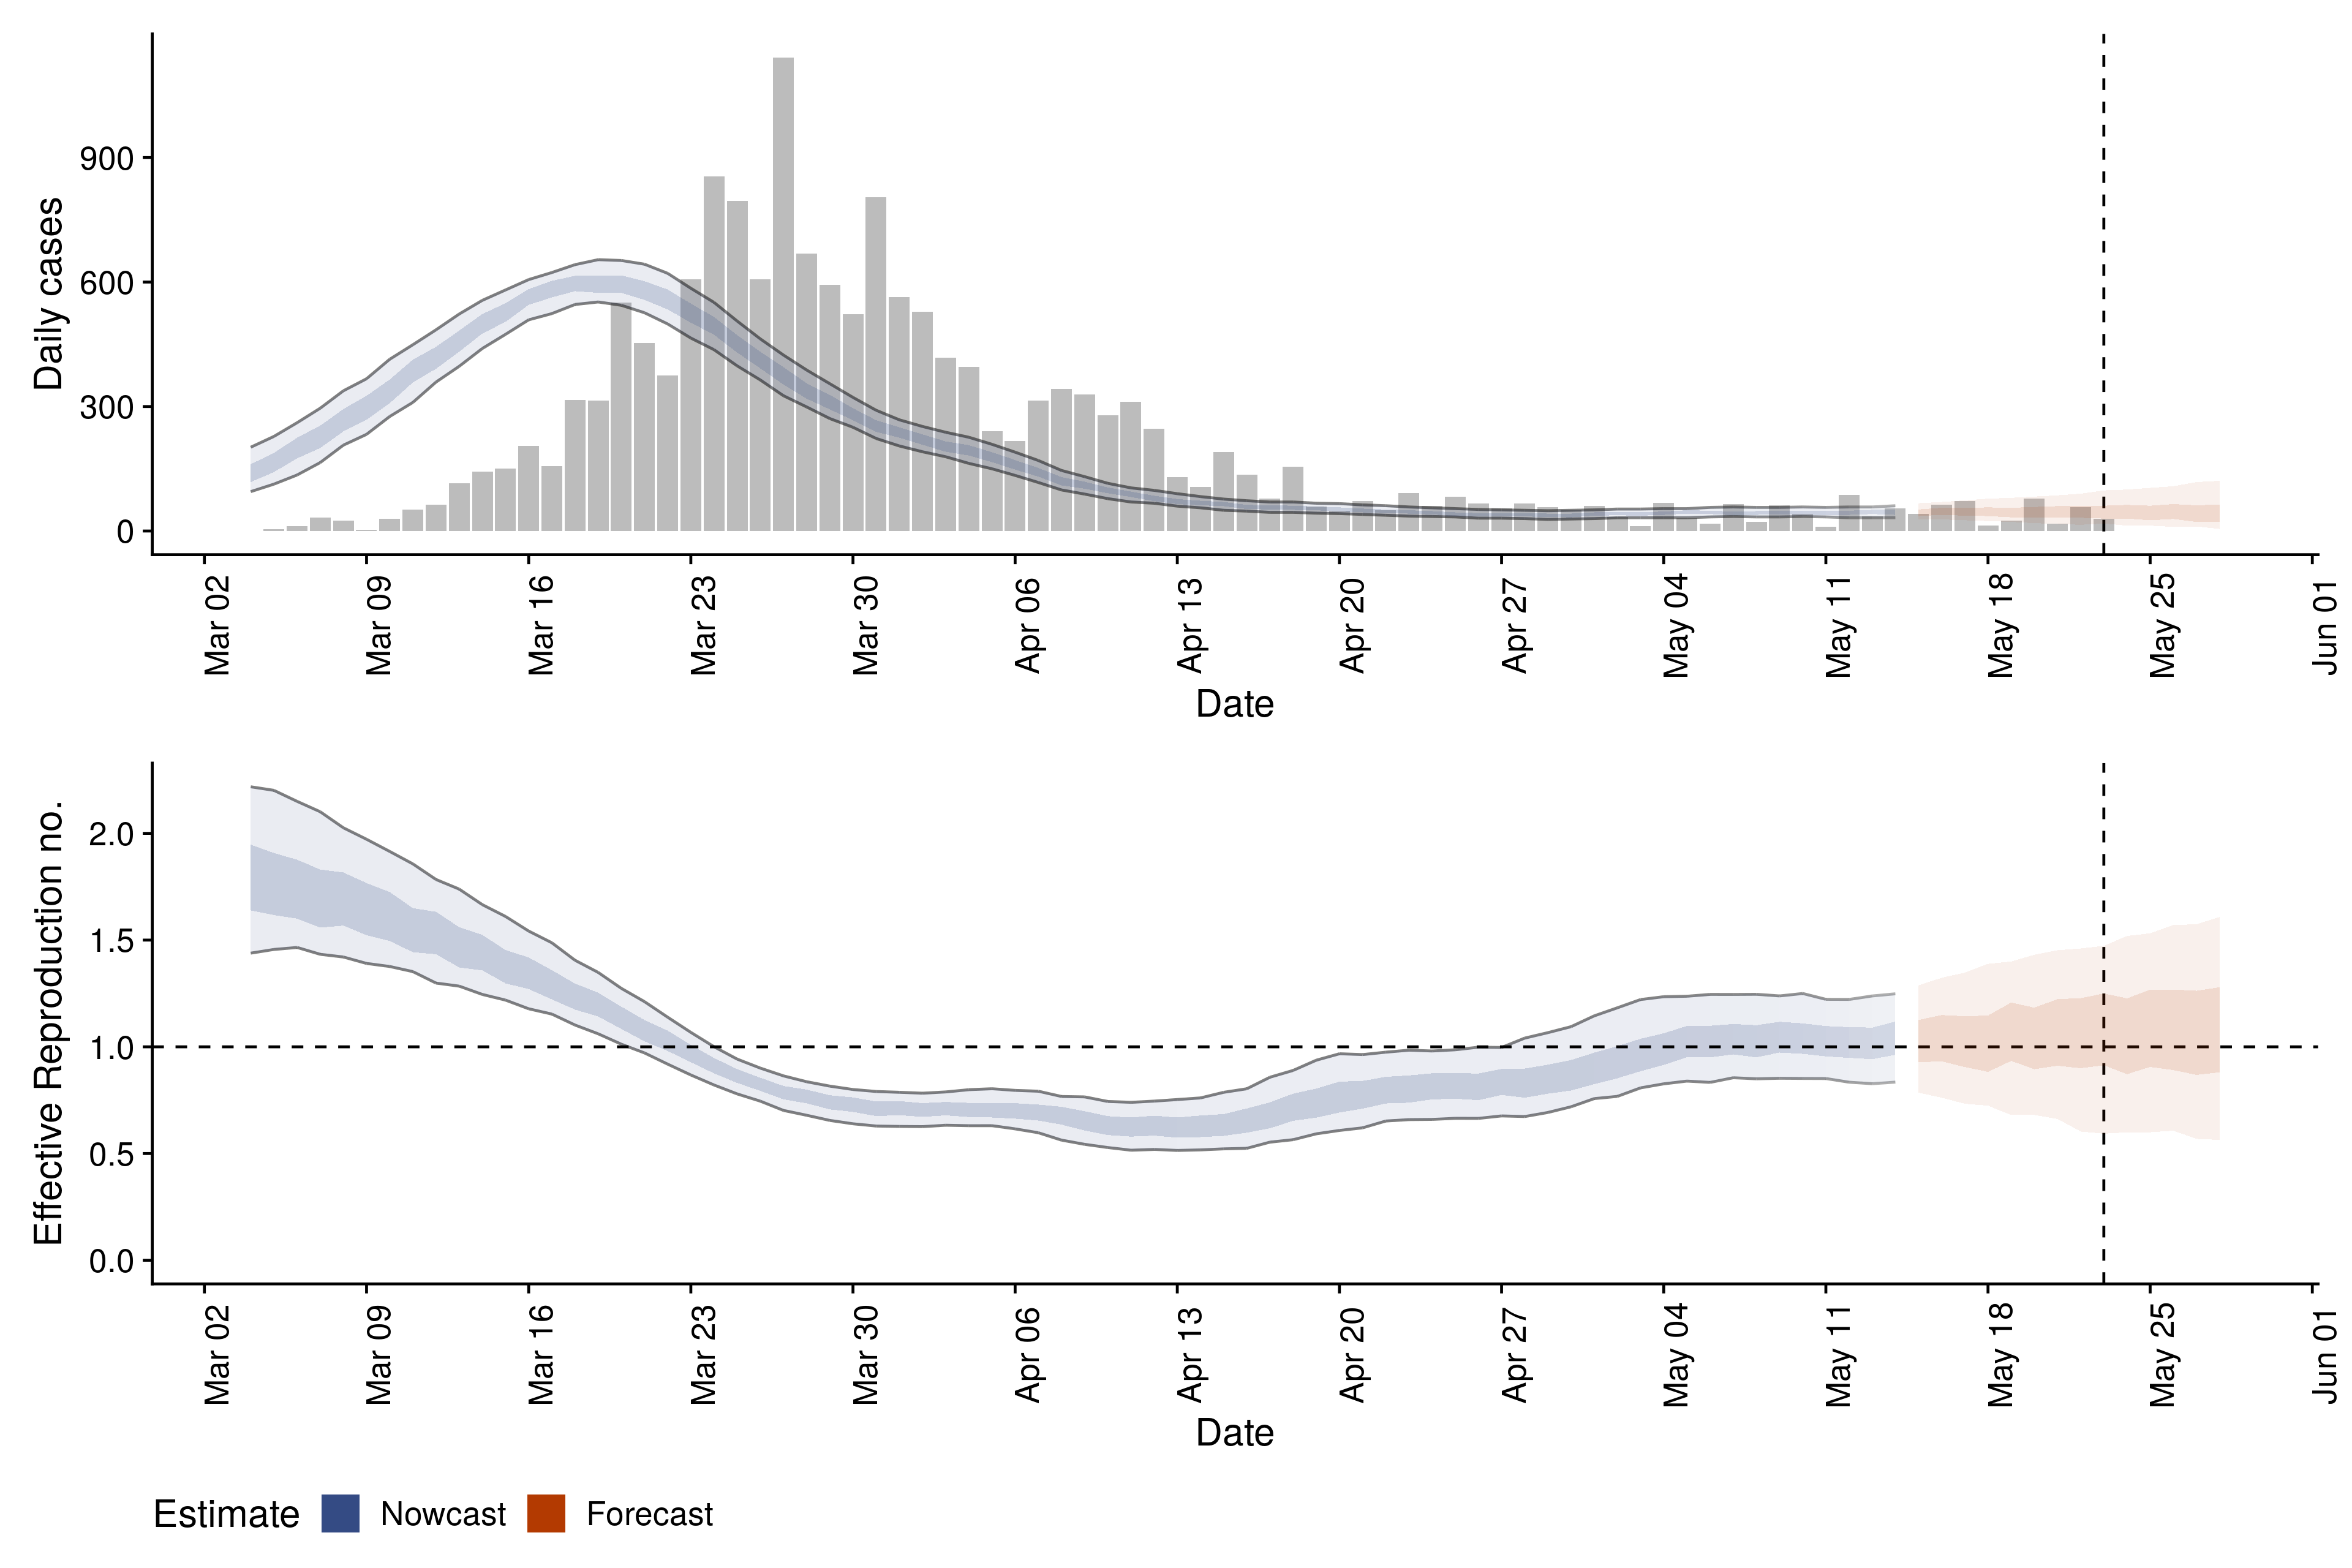
\includegraphics[width=0.9\linewidth]{figures/figure_1}

\emph{Figure 1: Confirmed cases by date of report (bars; top) and their
estimated date of infection (ribbon; top) and time-varying reproduction
number (bottom) in Austria. The light and dark blue ribbons show the
90\% and 50\% credible interval, respectively. The estimates were
generated on the 23rd May 2020. Due to the delay between being
infectious and becoming a confirmed case, the estimates lag behind the
present. Confidence in the estimated values is indicated by translucency
with increased translucency corresponding to increased uncertainty
deriving from right-truncation of reported cases in the estimate. The
forecast (red) is coloured differently from the nowcast (blue) to
indicate the drop in reliability when trying to forecast future cases.}

Sub-national breakdowns can highlight differences in how the outbreak is
progressing within a country (Figure 2) and are currently provided for 6
countries (Italy, Germany, United Kingdom, United States of America,
Brazil, India). For example, on the 23rd of May 2020 we estimated that
cases were likely decreasing in every country in the United Kingdom
except Northern Ireland where the estimate was classified as unsure.

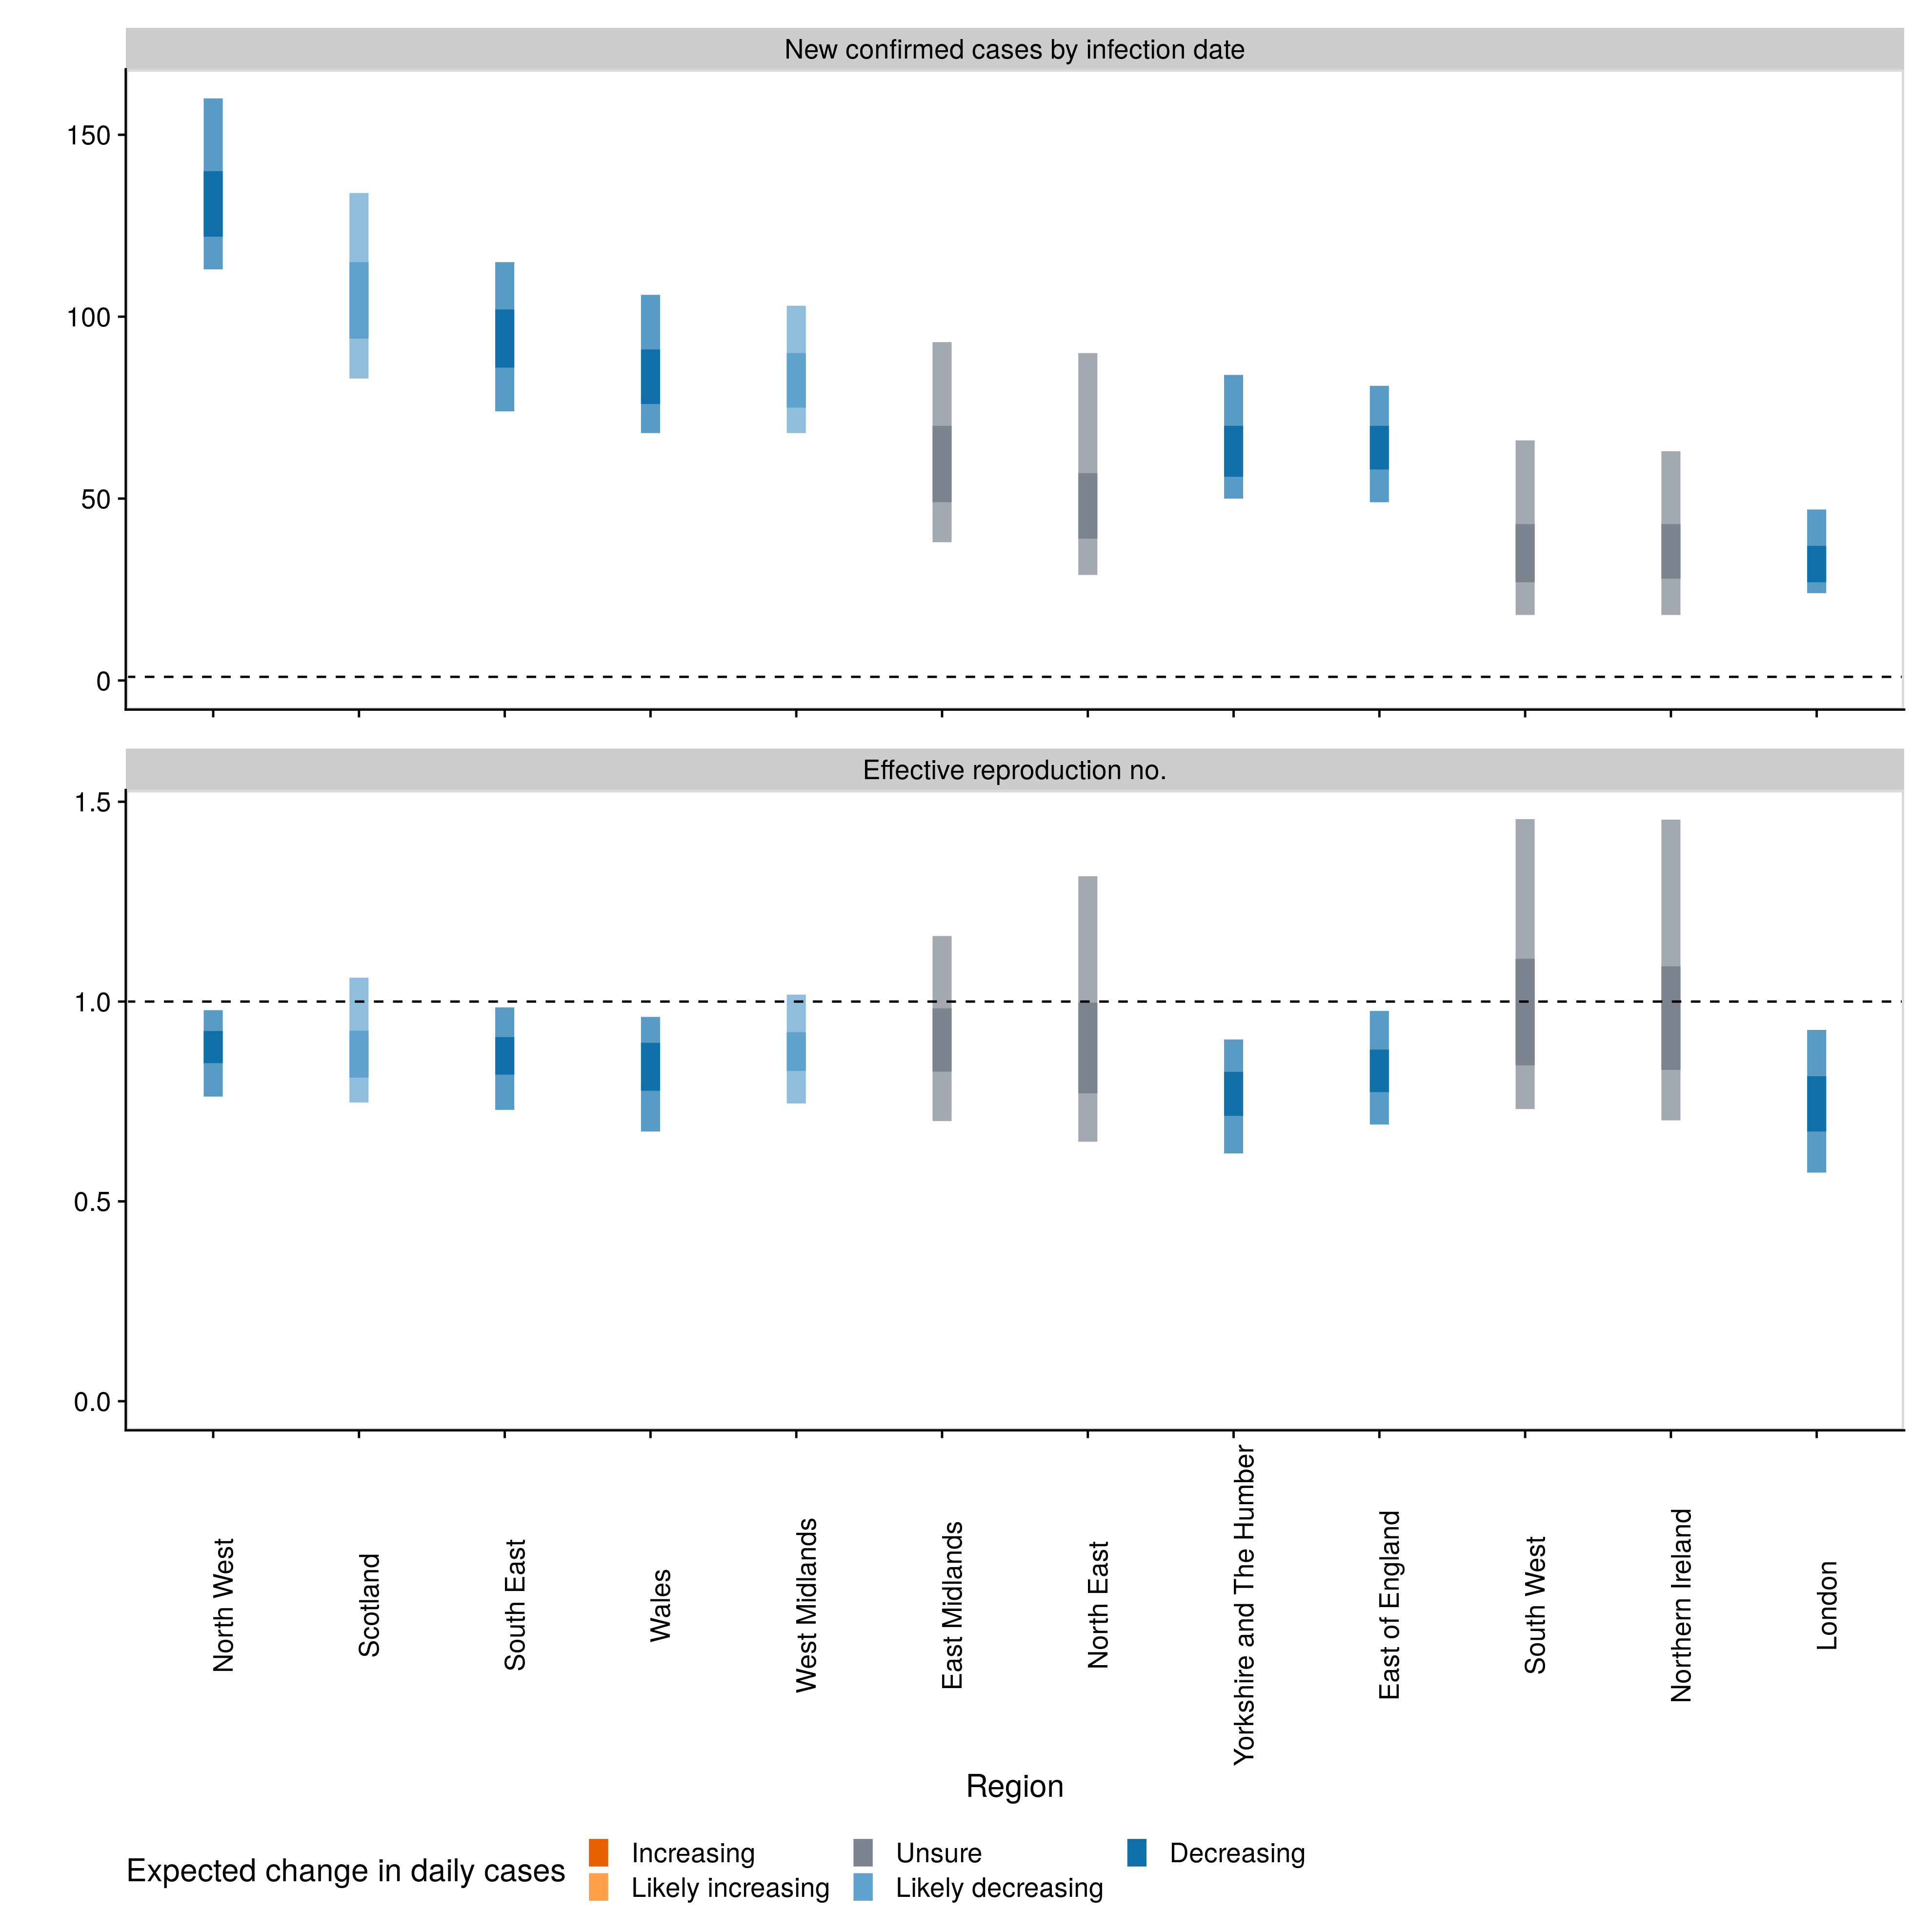
\includegraphics[width=0.9\linewidth]{figures/figure_2}

\emph{Figure 2: Estimates of numbers of cases that will be newly
infected on the date the estimate was made and that will end up being
reported (top panel), and the time-varying reproduction number (bottom
panel) across different nations/regions of the United Kingdom. Estimates
were produced on 23rd of May 2020. Nations/regions with fewer than 40
confirmed cases reported on a single day are not included in the
analysis.}

We present the nowcasting results on a map to effectively visualise
regional differences in transmission (Figure 3). This helps identify
areas where intervention policies are more effective at reducing
transmission than others, which can inform decision-making going
forwards.

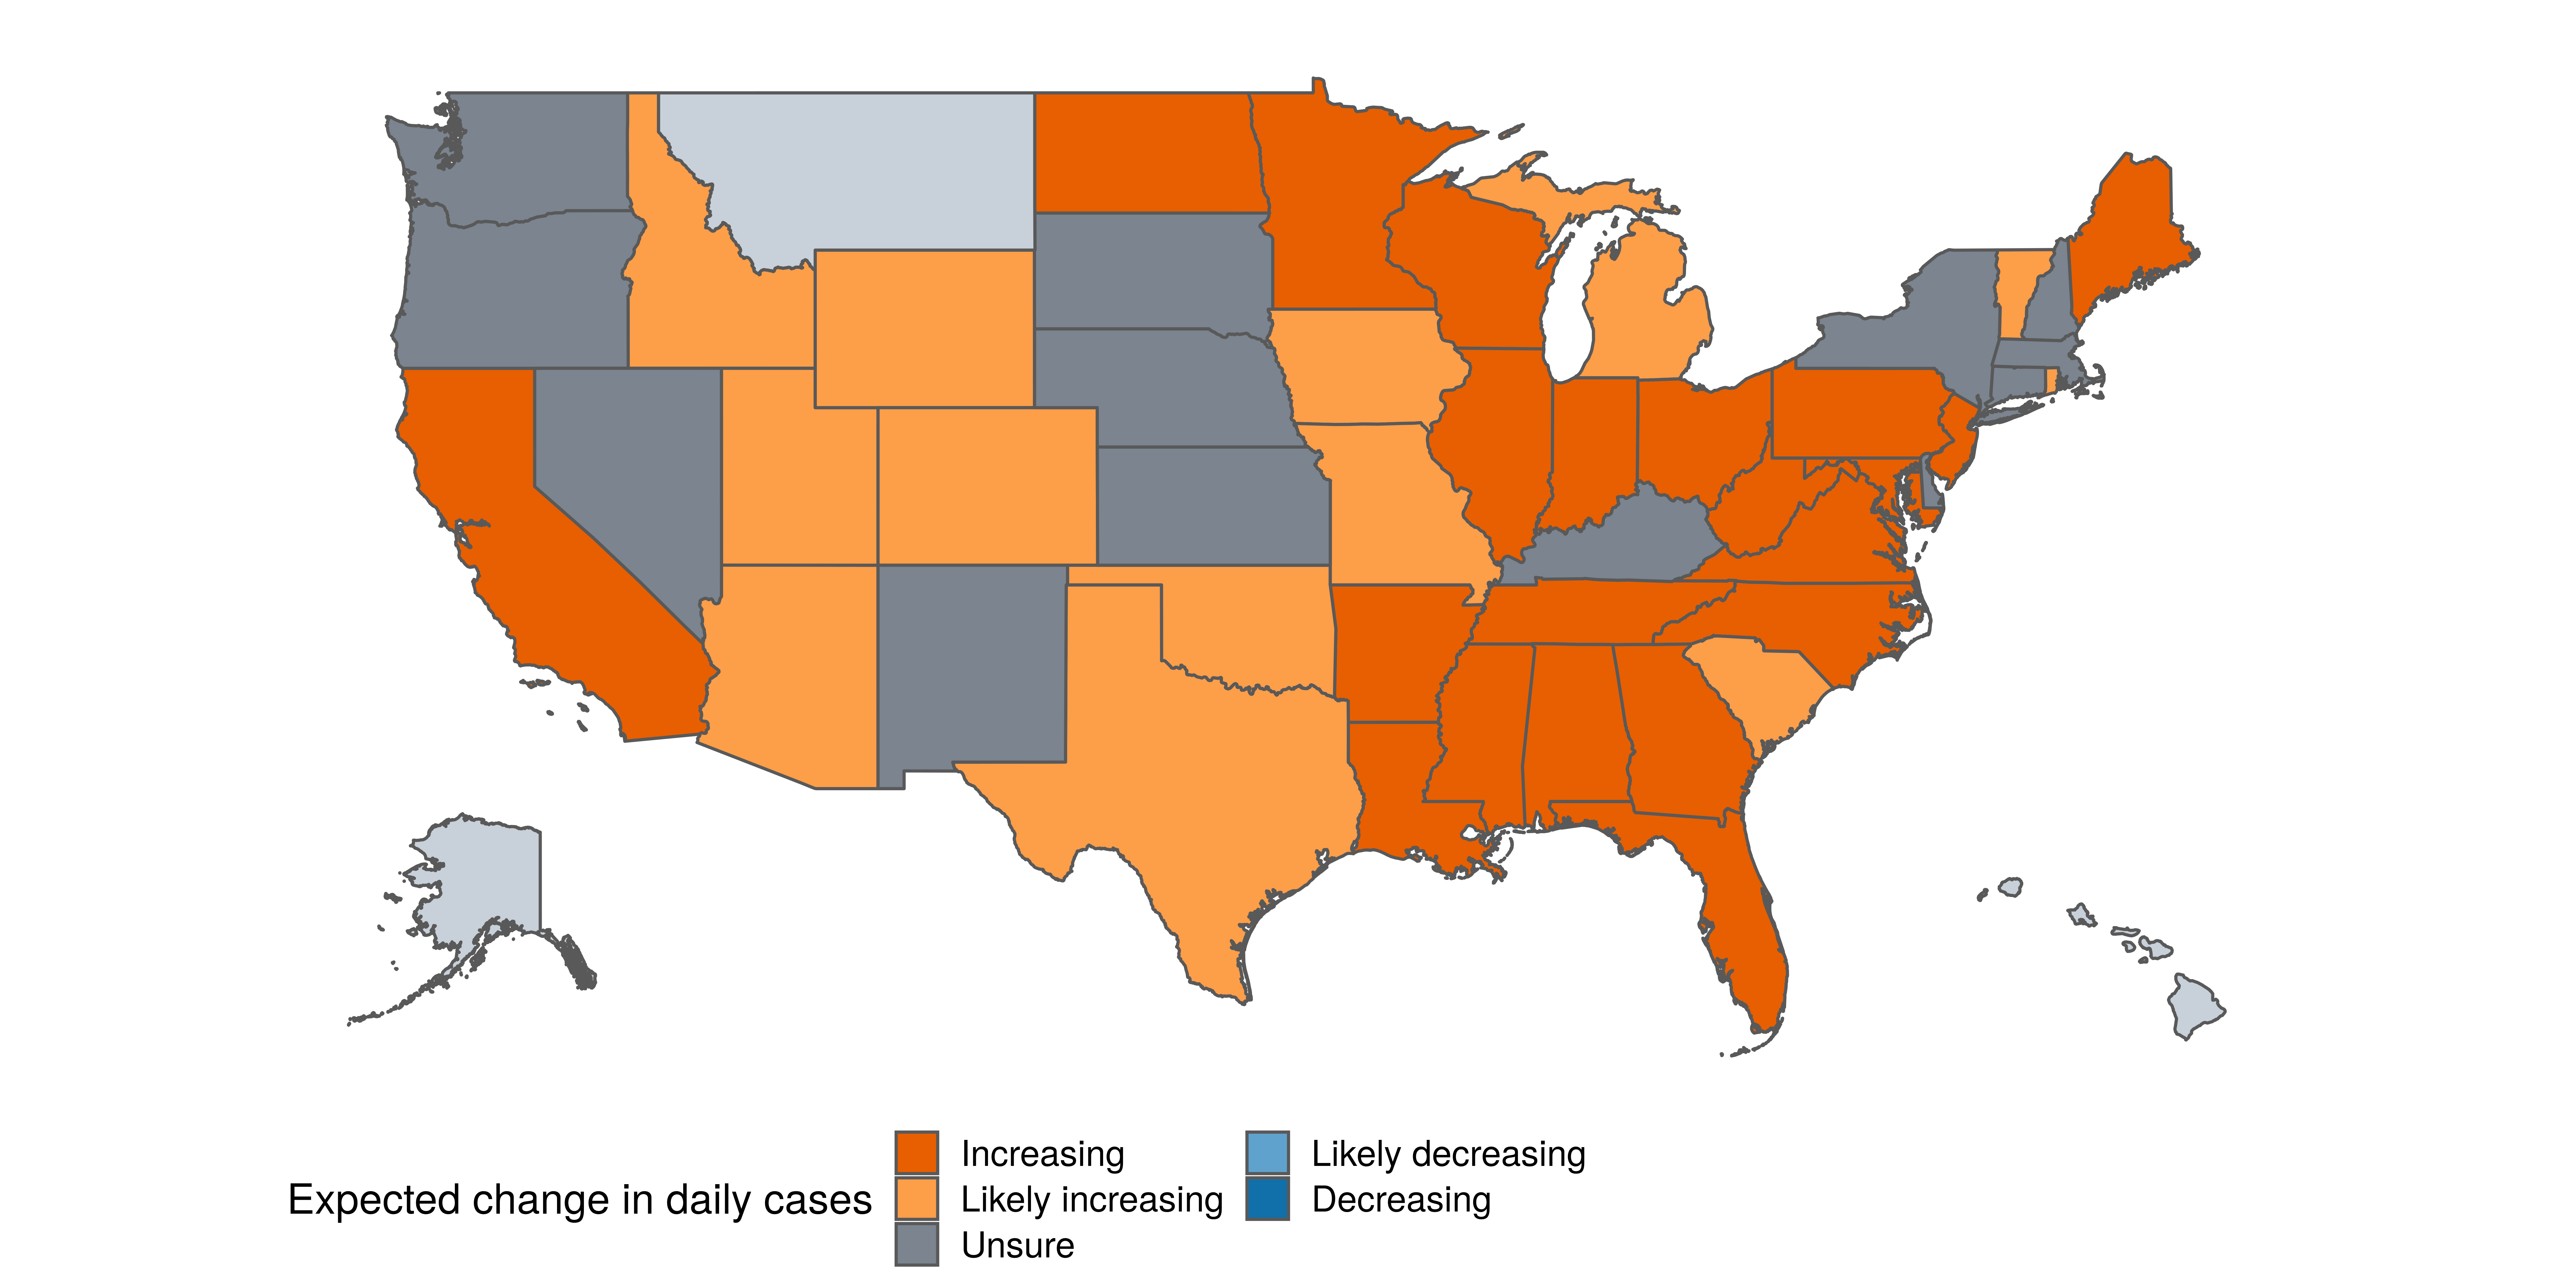
\includegraphics[width=0.9\linewidth]{figures/figure_3}

\emph{Figure 3: A map of the estimates of the expected change in daily
cases at the state level for the United States of America. Estimates
were produced on 23rd of May 2020. Regions with fewer than 40 confirmed
cases reported on a single day are not included in the analysis (light
grey).}

The methodology and toolset described here has also been used separately
to produce estimates of the time-varying reproduction number at the
state level in Australia, an example of how researchers and policymakers
can apply the methods to their own data {[}32{]}. This has an added
benefit of researchers being able to use generation time and delay
distributions derived from local data and not our global estimates. The
authors also use this tooling with confidential hospital admissions data
to generate estimates of the time-varying reproduction number for
policymakers in the United Kingdom.

\hypertarget{discussion}{%
\section{Discussion}\label{discussion}}

We provide a centralised resource, which generates comparable daily
estimates of the time-varying reproduction number and a daily nowcast of
the number of cases newly infected derived using a standardised method.
The estimates are free of any hypotheses about the impact of
interventions, since they are derived only from reported case counts and
an estimate of the generation time. We explicitly account for the delay
between infection and case notification and include all sources of
quantifiable uncertainty. This resource may be useful for policymakers
to track the progression of the COVID-19 outbreak and evaluate the
effectiveness of intervention measures. As new data become available, we
will include sub-national estimates for additional countries, and
provide additional support for public health agencies or researchers
interested in applying our methods to their data. We routinely utilise
our own tooling to provide estimates of the reproduction number in the
United Kingdom for policymakers using confidential hospital admissions
data.

There are several advantages associated with our approach. Firstly,
reported case counts are the only data required, which allows our
approach to be used in a wide variety of contexts. Secondly, we apply
the same methodology to all countries. This means that estimates can be
compared without having to consider differences in the underlying
methodology (even if differences in testing should still be accounted
for as discussed below). Finally, we have constructed our approach using
open source tools and all of our code, raw data, and results are
available online. This means our approach can be applied by others to
non-public data and be fully evaluated by end users.

Our approach is also subject to several limitation. Firstly, the model
requires that the proportion of infections that are notified is
constant. In other words, it requires consistency in the focus of the
surveillance method, level of effort spent on testing, and case
definition. Yet it is often the case that the level of under-reporting
in a country changes over the course of an outbreak {[}27{]}. However,
it should be noted that any changes in surveillance testing procedures
will only bias the estimates temporarily if they begin to remain
consistent again after they have changed. How long the bias remains in
the reproduction number estimates will depend on the serial generation
time and delay distributions, as well as the maximum window size used in
the reproduction number estimation process.

In addition, the model is limited by how representative the delay that
we use from infection to notification distribution is for a given
location. As there is limited data to assess this, we estimate a
bootstrapped global delay distribution using the combined data from
every country. In particular, the delay from onset to notification can
especially impact the upscaling of cases by date of onset that accounts
for cases that have onset but not yet been reported. If the true delay
from onset to notification for a given country is shorter than our
global delay, then we will overestimate onset case numbers, and vice
versa for true delays longer than the distribution we used.
Additionally, estimates of the reporting delay distribution are known to
be biased early in an epidemic and may vary over time {[}33{]}. However,
our use of a bootstrapped subsampling approach mitigates these issues by
allowing multiple delay distributions based on the observed data to be
considered at the cost of increasing uncertainty in our estimates.

Our model is also limited by the data avaliable to us. For example, the
publically available linelists contain little data on the importation
status of cases. This means that cases counts may be biased upwards by
attributing imported cases to local transmission. This bias is
particularly problematic when case counts are low. Unfortunately, in the
absence of data, this issue can only be explored via scenario analysis.
However, if and when data on the importation of cases is available, our
approach (via \emph{EpiEstim} {[}7{]}) supports adjusting for imported
cases.

As more data becomes available, future work should look to refine the
distributions used for generation time, incubation period, and the
report delay. There is also the potential to extend the present model to
account for overdispersion in the number of secondary infections
{[}34{]} and changes in the delay from onset to notification over the
course of an outbreak. Finally, there is scope to explore how outbreak
dynamics that differ among particular sub-populations, such as high-risk
COVID-19 patients, can bias overall reproduction number estimates.

Our approach, providing real-time estimates of the reproduction number,
serves as a valuable tool for decision makers looking to track the
course of COVID-19 outbreaks. The nowcasts explicitly account for
delays, using the same methodology across all countries and sub-national
regions. These reproduction number estimates can be used during the
initial stages of an outbreak to ascertain the likely outbreak
trajectory if no interventions have been implemented. They can also
provide real-time feedback on whether transmission is decreasing
following a particular intervention, or whether it is increasing
following the relaxing or lifting of current intervention measures. We
hope that our website and the related toolkit will provide a valuable
resource for devising strategies to contain COVID-19 outbreaks
worldwide.

\hypertarget{data-availability}{%
\subsection{Data availability}\label{data-availability}}

Latest data: \url{https://github.com/epiforecasts/covid}

Archived data at the time of publication:
\url{https://doi.org/10.5281/zenodo.3841818}

License: \href{https://opensource.org/licenses/MIT}{MIT}

\hypertarget{software-availability}{%
\subsection{Software availability}\label{software-availability}}

\hypertarget{development}{%
\subsubsection{Development}\label{development}}

\begin{itemize}
\tightlist
\item
  Website (Front-end): \url{https://github.com/epiforecasts/covid}
\item
  \emph{EpiNow} R package (R estimation, data processing, visualisation
  and reporting): \url{https://github.com/epiforecasts/EpiNow}
\item
  \emph{EpiSoon} R package (forecasting and case prediction from R
  trajectories): \url{https://github.com/epiforecasts/EpiSoon}
\item
  \emph{NCoVUtils} R package (data aggregation and processing):
  \url{https://github.com/epiforecasts/NCoVUtils}
\end{itemize}

\hypertarget{archived-at-the-time-of-publication}{%
\subsubsection{Archived at the time of
publication}\label{archived-at-the-time-of-publication}}

\begin{itemize}
\tightlist
\item
  Website: \url{https://doi.org/10.5281/zenodo.3841818}
\item
  \emph{EpiNow} R package {[}35{]}:
  \url{https://doi.org/10.5281/zenodo.3833806}
\item
  \emph{EpiSoon} R package {[}28{]}:
  \url{https://doi.org/10.5281/zenodo.3833807}
\item
  \emph{NCoVUtils} R package {[}36{]}:
  \url{https://doi.org/10.5281/zenodo.3833808}
\end{itemize}

License: \href{https://opensource.org/licenses/MIT}{MIT}

\hypertarget{acknowledgements}{%
\subsection{Acknowledgements}\label{acknowledgements}}

This project was enabled through access to the \textbf{MRC eMedLab
Medical Bioinformatics infrastructure}, supported by the \textbf{Medical
Research Council} (MR/L016311/1). Additional compute infrastructure and
support was provided by the \textbf{Met office}. We thank Venexia Walker
for comments on a version of this draft. The following authors were part
of the Centre for Mathematical Modelling of Infectious Disease 2019-nCoV
working group. Each contributed in processing, cleaning and
interpretation of data, interpreted findings, contributed to the
manuscript, and approved the work for publication: Samuel Clifford, Mark
Jit, Stéphane Hué, Eleanor M Rees, Petra Klepac, Damien C Tully, Rachel
Lowe, Kathleen O'Reilly, Nicholas G. Davies, Quentin J Leclerc, Arminder
K Deol, Gwenan M Knight, C Julian Villabona-Arenas, Fiona Yueqian Sun,
Emily S Nightingale, Alicia Rosello, Adam J Kucharski, Yang Liu, Billy J
Quilty, Matthew Quaife, Jon C Emery, Katherine E. Atkins, Simon R
Procter, W John Edmunds, Megan Auzenbergs, Christopher I Jarvis, David
Simons, Kiesha Prem, Graham Medley, Thibaut Jombart, Charlie Diamond,
Anna M Foss, Rein M G J Houben, Kevin van Zandvoort, Georgia R
Gore-Langton.

\hypertarget{funding}{%
\subsection{Funding}\label{funding}}

The following funding sources are acknowledged as providing funding for
the named authors. Alan Turing Institute (AE). This research was partly
funded by the Bill \& Melinda Gates Foundation (NTD Modelling Consortium
OPP1184344: CABP). DFID/Wellcome Trust (Epidemic Preparedness
Coronavirus research programme 221303/Z/20/Z: CABP). This research was
partly funded by the Global Challenges Research Fund (GCRF) project
`RECAP' managed through RCUK and ESRC (ES/P010873/1: AG). HDR UK
(MR/S003975/1: RME). Nakajima Foundation (AE). UK DHSC/UK Aid/This
research was partly funded by the National Institute for Health Research
(NIHR) using UK aid from the UK Government to support global health
research. The views expressed in this publication are those of the
author(s) and not necessarily those of the NIHR or the UK Department of
Health and Social Care (ITCRZ 03010: HPG). UK MRC (MC\_PC 19065: RME).
Wellcome Trust (206250/Z/17/Z: TWR; 208812/Z/17/Z: SFlasche;
210758/Z/18/Z: JDM, JH, NIB, SA, SFunk, SRM).

\hypertarget{references}{%
\section*{References}\label{references}}
\addcontentsline{toc}{section}{References}

\hypertarget{refs}{}
\leavevmode\hypertarget{ref-Linton:2020gg}{}%
1 Linton NM, Kobayashi T, Yang Y \emph{et al.} Incubation period and
other epidemiological characteristics of 2019 novel coronavirus
infections with right truncation: A statistical analysis of publicly
available case data. \emph{Journal of clinical medicine}
2020;\textbf{9}.

\leavevmode\hypertarget{ref-Cori:2017fg}{}%
2 Cori A, Donnelly CA, Dorigatti I \emph{et al.} Key data for outbreak
evaluation: Building on the ebola experience. \emph{Philosophical
transactions of the Royal Society of London Series B, Biological
sciences} 2017;\textbf{372}.

\leavevmode\hypertarget{ref-Mizumoto:2020ct}{}%
3 Mizumoto K, Kagaya K, Zarebski A \emph{et al.} Estimating the
asymptomatic proportion of coronavirus disease 2019 (covid-19) cases on
board the diamond princess cruise ship, yokohama, japan, 2020.
\emph{Eurosurveillance : bulletin Europeen sur les maladies
transmissibles = European communicable disease bulletin}
2020;\textbf{25}.

\leavevmode\hypertarget{ref-Donker:2011fk}{}%
4 Donker T, Boven M van, Ballegooijen WM van \emph{et al.} Nowcasting
pandemic influenza a/h1n1 2009 hospitalizations in the netherlands.
\emph{European journal of epidemiology} 2011;\textbf{26}:195--201.

\leavevmode\hypertarget{ref-vandeKassteele:2019cn}{}%
5 Kassteele J van de, Eilers PHC, Wallinga J. Nowcasting the number of
new symptomatic cases during infectious disease outbreaks using
constrained p-spline smoothing. \emph{Epidemiology (Cambridge, Mass)}
2019;\textbf{30}:737--45.

\leavevmode\hypertarget{ref-cori2013}{}%
6 Cori A, Ferguson NM, Fraser C \emph{et al.} A new framework and
software to estimate time-varying reproduction numbers during epidemics.
\emph{American Journal of Epidemiology} 2013;\textbf{178}:1505--12.
doi:\href{https://doi.org/10.1093/aje/kwt133}{10.1093/aje/kwt133}

\leavevmode\hypertarget{ref-THOMPSON2019100356}{}%
7 Thompson RN, Stockwin JE, Gaalen RD van \emph{et al.} Improved
inference of time-varying reproduction numbers during infectious disease
outbreaks. \emph{Epidemics} 2019;\textbf{29}:100356.
doi:\href{https://doi.org/https://doi.org/10.1016/j.epidem.2019.100356}{https://doi.org/10.1016/j.epidem.2019.100356}

\leavevmode\hypertarget{ref-Fraser:2007hf}{}%
8 Fraser C. Estimating individual and household reproduction numbers in
an emerging epidemic. \emph{PloS one} 2007;\textbf{2}:e758.

\leavevmode\hypertarget{ref-epinow2}{}%
9 Abbott S, Hellewell J, Hickson J \emph{et al.} EpiNow2: Estimate
real-time case counts and time-varying epidemiological parameters.
\emph{-} 2020;\textbf{-}:--.
doi:\href{https://doi.org/10.5281/zenodo.3957489}{10.5281/zenodo.3957489}

\leavevmode\hypertarget{ref-covidregionaldata}{}%
10 Abbott S, Sherratt K, Bevan J \emph{et al.} Covidregionaldata:
Subnational data for the covid-19 outbreak. \emph{-} 2020;\textbf{-}:--.
doi:\href{https://doi.org/10.5281/zenodo.3957539}{10.5281/zenodo.3957539}

\leavevmode\hypertarget{ref-EpiEstim}{}%
11 Cori A. \emph{EpiEstim: Estimate time varying reproduction numbers
from epidemic curves}. 2019.
\url{https://CRAN.R-project.org/package=EpiEstim}

\leavevmode\hypertarget{ref-forecastHybrid}{}%
12 Shaub D, Ellis P. \emph{ForecastHybrid: Convenient functions for
ensemble time series forecasts}. 2020.

\leavevmode\hypertarget{ref-ecdc_data}{}%
13 Disease Prevention EC for, Control. Download today's data on the
geographic distribution of covid-19 cases worldwide. 2020.
\url{www.ecdc.europa.eu/en/publications-data/download-todays-data-geographic-distribution-covid-19-cases-worldwide}

\leavevmode\hypertarget{ref-kraemer2020epidemiological}{}%
14 Xu B, Gutierrez B, Hill S \emph{et al.} Epidemiological data from the
nCoV-2019 outbreak: Early descriptions from publicly available data.
\url{http://virological.org/t/epidemiological-data-from-the-ncov-2019-outbreak-early-descriptions-from-publicly-available-data/337}

\leavevmode\hypertarget{ref-rstan}{}%
15 Stan Development Team. RStan: The r interface to stan.
2020.\url{http://mc-stan.org/}

\leavevmode\hypertarget{ref-Vehtari2016}{}%
16 Vehtari A, Gelman A, Gabry J. Practical bayesian model evaluation
using leave-one-out cross-validation and waic. \emph{Stat Comput}
2016;1--20.
doi:\href{https://doi.org/10.1007/s11222-016-9696-4}{10.1007/s11222-016-9696-4}

\leavevmode\hypertarget{ref-incubationperiod}{}%
17 Lauer SA, Grantz KH, Bi Q \emph{et al.} The incubation period of
coronavirus disease 2019 (covid-19) from publicly reported confirmed
cases: Estimation and application. \emph{Annals of Internal Medicine}
2020;\textbf{172}:577--82.

\leavevmode\hypertarget{ref-R}{}%
18 R Core Team. \emph{R: A language and environment for statistical
computing}. Vienna, Austria:: R Foundation for Statistical Computing
2019. \url{https://www.R-project.org/}

\leavevmode\hypertarget{ref-wallinga2004}{}%
19 Wallinga J, Teunis P. Different epidemic curves for severe acute
respiratory syndrome reveal similar impacts of control measures.
\emph{American Journal of Epidemiology} 2004;\textbf{160}:509--16.
doi:\href{https://doi.org/10.1093/aje/kwh255}{10.1093/aje/kwh255}

\leavevmode\hypertarget{ref-generationinterval}{}%
20 Ganyani T, Kremer C, Chen D \emph{et al.} Estimating the generation
interval for coronavirus disease (covid-19) based on symptom onset data,
march 2020. \emph{Eurosurveillance} 2020;\textbf{25}.

\leavevmode\hypertarget{ref-Imai:webreport3}{}%
21 Imai N, Cori A, Dorigatti I \emph{et al.} Report 3: Transmissibility
of 2019-nCoV.
\url{https://www.imperial.ac.uk/media/imperial-college/medicine/sph/ide/gida-fellowships/Imperial-2019-nCoV-transmissibility.pdf}

\leavevmode\hypertarget{ref-Abbott:2020hj}{}%
22 Abbott S, Hellewell J, Munday J \emph{et al.} The transmissibility of
novel coronavirus in the early stages of the 2019-20 outbreak in wuhan:
Exploring initial point-source exposure sizes and durations using
scenario analysis. \emph{Wellcome open research} 2020;\textbf{5}:17.

\leavevmode\hypertarget{ref-NOUVELLET201829}{}%
23 Nouvellet P, Cori A, Garske T \emph{et al.} A simple approach to
measure transmissibility and forecast incidence. \emph{Epidemics}
2018;\textbf{22}:29--35.
doi:\href{https://doi.org/https://doi.org/10.1016/j.epidem.2017.02.012}{https://doi.org/10.1016/j.epidem.2017.02.012}

\leavevmode\hypertarget{ref-gneiting_strictly_2007}{}%
24 Gneiting T, Raftery AE. Strictly proper scoring rules, prediction,
and estimation. \emph{Journal of the American Statistical Association}
2007;\textbf{102}:359--78.
doi:\href{https://doi.org/10.1198/016214506000001437}{10.1198/016214506000001437}

\leavevmode\hypertarget{ref-jordan_evaluating_2019}{}%
25 Jordan A, Krüger F, Lerch S. Evaluating probabilistic forecasts with
scoringRules. \emph{Journal of Statistical Software} 2019;\textbf{90}.
doi:\href{https://doi.org/10.18637/jss.v090.i12}{10.18637/jss.v090.i12}

\leavevmode\hypertarget{ref-Park2019}{}%
26 Park SW, Champredon D, Weitz JS \emph{et al.} A practical
generation-interval-based approach to inferring the strength of
epidemics from their speed. \emph{Epidemics} 2019;\textbf{27}:12--8.
doi:\href{https://doi.org/https://doi.org/10.1016/j.epidem.2018.12.002}{https://doi.org/10.1016/j.epidem.2018.12.002}

\leavevmode\hypertarget{ref-Russell:BFVkJ6lQ}{}%
27 Russell TW. Using a delay-adjusted case fatality ratio to estimate
under-reporting.
\url{https://cmmid.github.io/topics/covid19/severity/global_cfr_estimates.html}

\leavevmode\hypertarget{ref-episoon}{}%
28 Abbott S, Hellewell J, Bosse N \emph{et al.} \emph{EpiSoon: Forecast
cases using reproduction numbers}. 2020.
\url{https://epiforecasts.io/EpiSoon}

\leavevmode\hypertarget{ref-scoringrules}{}%
29 Jordan A, Kruger F, Lerch S. Evaluating probabilistic forecasts with
scoringRules. \emph{Journal of Statistical Software}
2019;\textbf{90}:1--37.
doi:\href{https://doi.org/10.18637/jss.v090.i12}{10.18637/jss.v090.i12}

\leavevmode\hypertarget{ref-scoringutils}{}%
30 Bosse N. \emph{Scoringutils: A collection of proper scoring rules and
metrics to assess predictions}. 2020.
\url{https://github.com/epiforecasts/scoringutils}

\leavevmode\hypertarget{ref-Funk2019cc}{}%
31 Funk S, Camacho A, Kucharski AJ \emph{et al.} Assessing the
performance of real-time epidemic forecasts: A case study of ebola in
the western area region of sierra leone, 2014-15. \emph{PLoS
computational biology} 2019;\textbf{15}:e1006785--17.

\leavevmode\hypertarget{ref-Price:2020dh}{}%
32 Price DJ, Shearer FM, Meehan MT \emph{et al.} Early analysis of the
australian covid-19 epidemic. 2020;1--22.

\leavevmode\hypertarget{ref-Britton:2019gf}{}%
33 Britton T, Scalia Tomba G. Estimation in emerging epidemics: Biases
and remedies. \emph{Journal of the Royal Society, Interface}
2019;\textbf{16}.

\leavevmode\hypertarget{ref-10.12688ux2fwellcomeopenres.15842.1}{}%
34 Endo A, Abbott S, Kucharski AJ \emph{et al.} Estimating the
overdispersion in covid-19 transmission using outbreak size outside
china {[}version 1; peer review: 1 approved{]}. \emph{Wellcome open
research} 2020;\textbf{5}.

\leavevmode\hypertarget{ref-epinow}{}%
35 Abbott S, Hellewell J, Munday J \emph{et al.} \emph{EpiNow: Estimate
realtime case counts and time-varying epidemiological parameters}. 2020.
\url{https://github.com/epiforecasts/EpiNow}

\leavevmode\hypertarget{ref-NCoVUtils}{}%
36 Abbott S, Hellewell J, Munday JD \emph{et al.} NCoVUtils: Utility
functions for the 2019-ncov outbreak. \emph{-} 2020;\textbf{-}:--.
doi:\href{https://doi.org/10.5281/zenodo.3635417}{10.5281/zenodo.3635417}

\end{document}
